\documentstyle[12pt,thesis]{ireport}
\date{\today}
\author{Brian S. Corbin}
\advisor{Dr$.$ D$.$E$.$ Stevenson}
\title{CORBin:  A System Providing CORBA Support to the Standard ML of New Jersey Compiler}
\department{Computer Science}
\dissertation{Thesis}
\degree{Master of Science}
\subdate{May 4, 2001}
\semester{May 2001}


\input{psfig.sty}
% use Section{}, SubSection{} and SubSubSection{} instead of
%    standard section{}, subsection{} and subsubsection{} to
%     obtain headings in the form "1.3: My heading"

%\def\figline{\rule{\textwidth}{0.3mm}}
%\def\mysection#1#2{\Section{#1}\label{#2}\input{#2}}

\def\CPP{C\raise.22ex\hbox{{\footnotesize +}}\raise.22ex\hbox{\footnotesize +}}
\def\BCPP{C\raise.22ex\hbox{{\footnotesize \bf +}}\raise.22ex\hbox{\footnotesize \bf +}}

\def\figline{\rule{\textwidth}{0.3mm}}

%\usepackage{keywords}
%\usepackage{epsfig}

\begin{document}

%%%%%%%%%%%%%%%%%%%%%%%%%Signature Page%%%%%%%%%%%%%%%%%%%%%%%%%%%%%%%%%
\makesignature
\preliminaries
\maketitle

%%%%%%%%%%%%%%%%%%%%%%%The ABSTRACT%%%%%%%%%%%%%%%%%%%%%%%%%%%%%%%%%%%%%
\begin{abstract}
\input{abstract}
\end{abstract}

%%%%%%%%%%%%%%%%%%%%%%%%%The DEDICATION%%%%%%%%%%%%%%%%%%%%%%%%%%%%%%%%%
\begin{dedication}

This work is dedicated to Mrs$.$ Fred V$.$ Brown.
Her \emph{Prayer Boots} have provided me with the 
dedication and determination to produce this thesis. 

\end{dedication}
%%%%%%%%%%%%%%%%%%%%%%%%Acknowledgements%%%%%%%%%%%%%%%%%%%%%%%%%%%%%%%%
\begin{acknowledgments}

GOD:  Thank you. 

I would like to thank Dr$.$ Steve Stevenson for the opportunity to 
pursue this research and paper.  Dr$.$ Stevenson's willingness to allow me 
freedom to explore various ideas made this experience a very beneficial 
one.  I'd also like to thank Dr$.$ Mike Westall for believing in me.
Without Dr$.$ Westall, this work would have never been realized. 
The paper and research in it's final form would not have been possible 
without the help of Dr$.$ Brian Malloy and Dr$.$ Sandee Hedetniemi.  I 
appreciate their advice and support. I'd also like to thank the computer
science professors that I was fortunate enough to work with while an undergrad
at Wofford College:  Dr$.$ Dan W$.$ Olds, Dr$.$ Angela Shiflet, Dr$.$ Ben Varn, and 
Dr$.$ Dan W$.$ Welch.  The four of you provided me with an excellent foundation 
in computing.  A special thanks to all of the 
undergraduates that have allowed me the opportunity to share my love of 
computer programming with them.  The many hours spent helping undergraduate 
computer science students in G-29 Jordan Hall will be one of my most 
cherished memories of my time at Clemson University. 
I'd be at fault if I did not give a great thanks to my friends and family.
My family has provided continued support throughout my educational career 
and for that I am forever indebted.  God has truly blessed me with a great 
family. Mom and Dad:  Thanks for all of the support! 
Mom: "I love Mooch, too!"   Dad: "Page me if you need something!"
A special thank you to my friends who kept me laughing via email 
when times were dark.  Thanks to all of my peers for allowing me to work
with the greatest minds in the computing world today.  Thanks to 
COMET3.CS.CLEMSON.EDU for allowing me to utilize her CPU cycles. 
Lastly, thanks go out to "Stone Cold" Steve Austin 
for showing me that hard-work, determination, and enthusiasm can make a 
world of difference.  And that's the bottom line...cause it's "Miller Time!"


\end{acknowledgments}

%%%%%%%%%%%%%%%%%%%%%%%Table of Contents%%%%%%%%%%%%%%%%%%%%%%%%%%%%%%%%
\tableofcontents
%%%%%%%%%%%%%%%%%%%%%%%List of Figures%%%%%%%%%%%%%%%%%%%%%%%%%%%%%%%%%%
\listoffigures
\body

%%%%%%%%%%%%%%%%%%%%%%%%%Introduction%%%%%%%%%%%%%%%%%%%%%%%%%%%%%%%%%%%
\chapter{\uppercase{Introduction}}
\label{intro}
\input{intro}

%%%%%%%%%%%%%%%%%%%%%%%%%Background%%%%%%%%%%%%%%%%%%%%%%%%%%%%%%%%%%%%%
\chapter{\uppercase{Background}}
\label{back}

In this chapter, we provide background information related to several topics 
discussed in this paper. 

\section*{\underline{CORBA: Common Object Request Broker Architecture}}
\addcontentsline{toc}{section}{CORBA: Common Object Request Broker Architecture}

In an effort to provide a solution to the interoperability problem, the Object 
Management Group (OMG) created the Common Object Request Broker Architecture
(CORBA).  \cite{siegel}  CORBA is OMG's open, vendor-independent architecture 
and infrastructure that computer applications use to work together over networks.
\cite{omg} By using the Internet Inter ORB Protocol (IIOP), a CORBA-based program 
from any vendor, on almost any computer, operating system, programming language, 
and network, can inter-operate with a CORBA-based program from the same or another 
vendor, on almost any other computer, operating system, programming language, 
and network. \cite{omg} Since CORBA is based upon object orientation, you must 
define each CORBA object's interface in OMG's Interface Definition Language (IDL). 
This fixes the operations the CORBA object will perform, and the input and output 
parameters each will accept.\cite{siegel} This interface definition is independent 
of your programming language. \cite{omg} The interface to each CORBA object is 
defined very strictly. But, in contrast, the implementation of a CORBA object
is hidden from the rest of the system behind a boundary that the client may not 
cross. Clients access CORBA objects only through their advertised interface, 
invoking only those operations that the object chooses to expose, with only 
those parameters that are included in the invocation. \cite{omg}

In order to create a CORBA-based application, you must compile the IDL 
specification for the objects you wish to utilize.  This compilation will 
generate IDL stubs and skeletons for the objects defined within the IDL
specification.  Once the stubs and skeletons have been generated, the 
object can be implemented and a client application can be written to 
utilize the functionality of the object.  
These IDL stubs and skeletons act as proxies for the client application and 
object implementation.\cite{omg} 
Figure \ref{RequestPassing} illustrates the use of IDL stubs and skeletons as 
a client application's request is being passed to a CORBA object.  
 
\begin{figure}
\begin{center}
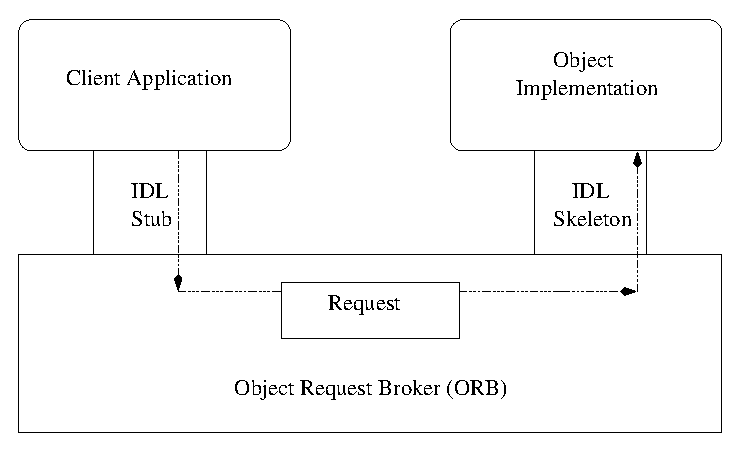
\psfig{file=Figures/RequestPassing.eps}
\leavevmode
\caption{\em{A request passing from a client application to an object implementation using the same ORB}.}
\figline
         \label{RequestPassing}
\end{center}
\end{figure}

When CORBA is being used to communicate between objects that reside 
on the same computer, the scenario depicted in figure \ref{RequestPassing}
could accurately illustrate the necessary path of communication for an 
invocation request.  However, when objects reside on remote computers, 
communication must take place between multiple ORBs.  The scenario where a 
client invokes an operation on a remote CORBA object is illustrated in 
figure \ref{ORB2ORB}.   
Since the standard Internet Inter ORB Protocol is being used to communicate 
between the ORBs, the ORBs can be from different vendors and still inter-operate
with ease.   
For more information on CORBA, the author recommends {\em{CORBA 3: Fundamentals
and Programming}} by Jon Siegel, PhD.  
\begin{figure}
\begin{center}
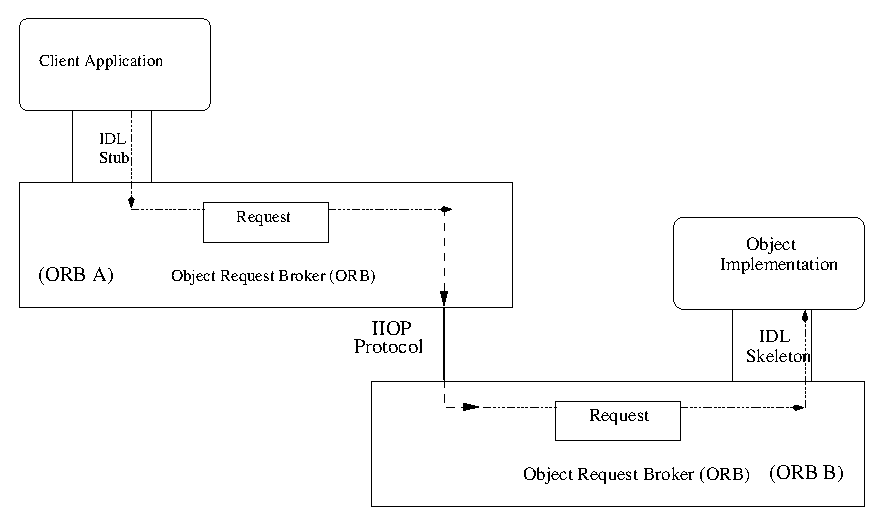
\psfig{file=Figures/ORB2ORB.eps}
\leavevmode
\caption{\em{A request passing from a client application using ORB A to an object implementation using ORB B}.}
\figline
         \label{ORB2ORB}
\end{center}
\end{figure}


\section*{\underline{IDL: Syntax and Semantics}}
\addcontentsline{toc}{section}{IDL: Syntax and Semantics}


The Object Management Group's Interface Definition Language (IDL) is a 
subset of the \CPP \space programming language with additional keywords 
added for distributed concepts.  IDL does not include any algorithmic 
structures or variables.  While IDL syntax is similar to \CPP , the 
semantics of the languages are very different.  
\cite{siegel}  IDL is the strongly typed language used to 
provide a very strict definition of CORBA objects.   This strict definition 
is used to {\em{map}} IDL to a programming language so a programmer 
can implement and communicate with CORBA objects.  
IDL defines basic, constructed, and template types.  \cite{siegel}
The basic IDL types are listed in figure \ref{BasicIDLTypes}.  
In addition to these basic types, IDL offers structures and arrays.
In order to ensure interoperability, OMG's official language mappings 
map every IDL type to something in every mapped language.  \cite{siegel}
For the most complete and current information related to IDL, please 
refer to OMG's Official Website: {\em{http://www.omg.org}}. The IDL grammar 
, according to the CORBA 2$.$4 specification, is included in the appendix. 

\begin{figure}
\begin{center}
\psfig{file=Figures/BasicIDLTypes.eps}
\leavevmode
\caption{\em{The Basic IDL Types}.}
\label{BasicIDLTypes}
\end{center}
\end{figure}




\section*{\underline{ORBit}}
\addcontentsline{toc}{section}{ORBit}


ORBit is a CORBA 2.2-compliant Object Request Broker (ORB) featuring 
mature C and Perl bindings. Bindings in various degrees of completeness 
are also available for C++, Lisp, Pascal, Python, Ruby, and TCL; others 
are in-progress. It supports POA, DII, DSI, TypeCode, Any, IR and IIOP. 
Optional features including INS and threading are available. ORBit is 
engineered for the desktop workstation environment, with a focus on 
performance, low resource usage, and security.  The core ORB is 
written in C, and runs under Linux, UNIX and Microsoft Windows. ORBit is 
developed and released as open source software under GPL/LGPL.  
It is supported by Red Hat and Ximian as part of the 
GNOME project.\cite{orbit} For more information on ORBit, please refer to 
the ORBit website: {\em{http://orbit-resource.sourceforge.net/}}.




\section*{\underline{The SML/NJ C Interface}}
\addcontentsline{toc}{section}{The SML/NJ C Interface}


Since it is common to distribute reusable software modules in the form of 
C language function libraries, a C foreign function interface was 
created for the SML/NJ compiler. \cite{lorenz}  This interface comes in two 
parts: a library of C functions in the SML/NJ runtime system and an SML/NJ
library that must be explicitly loaded into the top-level environment of 
SML/NJ prior to foreign function application. \cite{lorenz} This interface 
also allows function pointers, representing ML functions, to be passed to 
C functions as parameters so that ML functions may be called from C.   
The SML/NJ library portion of the interface provides ML data types representing
the types available in the C programming language.  These data types allow the 
ML programmer to easily pass data from ML to C and vice-versa.



\section*{\underline{The ML Type System}}
\addcontentsline{toc}{section}{The ML Type System}

ML is a strongly-typed language, meaning that all values and 
variables have an associated type that can be determined at 
compile time. \cite{ullman} A value of one type may not be 
assigned to a variable of another type.  \cite{ullman} 
ML's strong typing is a valuable debugging aid, since it 
allows many errors to be caught by the compiler, rather 
than resulting in very mysterious errors when the program
is executed.  Although most other strongly typed languages 
require an explicit declaration of the type of every 
variable, ML will try to figure out the unique type of each    
variable and will only require a declaration for a variable 
when it is impossible to deduce its type.  \cite{ullman}






%%%%%%%%%%%%%%%%%%%%%%%%%CORBin Discussion%%%%%%%%%%%%%%%%%%%%%%%%%%%%%%
\chapter[\uppercase{The C ORB Interface System for the SML/NJ Compiler}]%
        {\uppercase{CORBin: The C ORB Interface System for the SML/NJ Compiler}}
\label{implement}

The C ORB Interface System (CORBin) consists of two components: an IDL compiler, 
corbin-idl,  and a library of C functions.   The sections in this chapter 
discuss these two parts of the C ORB Interface system in detail. 

\section*{\underline{The IDL Compiler:  corbin-idl}}
\addcontentsline{toc}{section}{The IDL Compiler:  corbin-idl}

The corbin-idl compiler, like any IDL compiler, is used to produce stubs and 
skeletons from an IDL specification.   Corbin-idl parses IDL specifications
according the the IDL grammar found in the CORBA 2$.$4 specification.
Since corbin-idl relies upon ORBit to do the actual marshalling and 
de-marshalling of parameters for operation invocations on CORBA objects, 
corbin-idl generates C functions that {\em{wrap}} the functions generated 
by orbit-idl, the IDL compiler for ORBit.   In addition to generating 
C code, corbin-idl generates ML code that works with the SML/NJ C 
interface. \cite{lorenz} This ML code must be explicitly loaded into 
the top-level environment of SML/NJ before CORBin related functions 
may be used. The subsections that follow discuss the process of 
stub and skeleton generation for the C ORB Interface. 

\subsection*{IDL stubs}
\addcontentsline{toc}{subsection}{IDL stubs} 

There are four key steps involved in the corbin-idl stub generation process.
Since corbin-idl acts as an interface to ORBit, the first step in this 
process is to generate C functions that wrap the IDL stub functions generated 
by ORBit's IDL compiler, orbit-idl.   
Suppose the IDL specification defined in figure \ref{foointerface} 
is given as input to corbin-idl.
\begin{figure*}[t]
\singlespace
\begin{verbatim}

     interface foo {

          long bar(in long x); 

     };

\end{verbatim}
\doublespace
\caption {\em {IDL Specification for a CORBA object called foo}.}
\figline
        \label{foointerface}
\end{figure*}
Once corbin-idl has parsed this IDL specification, it generates a 
C function to wrap the stub function for the bar operation. 
This C function is illustrated in figure \ref{CStubWrapper}.
\begin{figure*}[t]
\singlespace
\begin{verbatim}

     long CORBin_foo_bar(CORBA_Object obj, long x)
     {
          return foo_bar(obj, x, &ev);
     }
 
\end{verbatim}
\doublespace
\caption {\em {C function generated by corbin-idl to invoke the bar operation of a foo object}.}
\figline
        \label{CStubWrapper}
\end{figure*}

Because CORBin utilizes the SML/NJ C foreign function interface, 
corbin-idl must generate C macros to explicitly define the stub function 
wrappers in the SML/NJ runtime system.
The C Macro generated for the CORBin\_foo\_bar function 
is shown in figure \ref{CStubMacro}.
This macro is appended to a C header file that is included during the 
building process of the SML/NJ runtime system.  This is done so that the 
CORBin\_foo\_bar function can be made available to the ML programmer
in the top-level environment of SML/NJ.
\begin{figure*}[t]
\singlespace
\begin{verbatim}

C_CALLS_CFUNC("CORBin_foo_bar",CORBin_foo_bar,long ,(void *, long ))
 
\end{verbatim}
\doublespace
\caption {\em {C Macro to explicitly define the CORBin\_foo\_bar function in the SML/NJ runtime system}.}
\figline
        \label{CStubMacro}
\end{figure*}

The third step in the corbin-idl stub generation process is to execute 
orbit-idl so that IDL stubs will be generated to use ORBit.  By doing this,
the details involved with the marshalling and de-marshalling of 
parameters during operation invocations are left to the functions generated
by orbit-idl.  Therefore, corbin-idl is only concerned with passing data 
from ML to C when an operation is invoked on a CORBA object from ML. 
Once the data has been passed to the appropriate C function, it is transfered
to the CORBA object's operation via ORBit functionality.   

The final step of this process involves the generation of ML code to 
explicitly load the SML/NJ C Interface into the top-level environment 
of SML/NJ so that the ML programmer can implement and communicate with the 
CORBA objects defined in the IDL specification.   During this step, corbin-idl
generates a signature and a value/function pair in ML for each stub wrapper
function generated.  The signature generated for foo's bar operation is shown
in figure \ref{MLStubSig} and the value/function pair is shown in figure 
\ref{MLStubValFun}.  This ML code explicitly defines the parameter and return
types for the stub wrapper functions generated by corbin-idl.   
Once this code has been loaded into the top-level environment of SML/NJ, 
the ML programmer can call the functions corbin-idl has created.  
\begin{figure*}[t]
\singlespace
\begin{verbatim}

     val CORBin_foo_bar : caddr  * Word32.word  -> Word32.word

\end{verbatim}
\doublespace
\caption {\em{ML signature for the CORBin\_foo\_bar function}.}
\figline
        \label{MLStubSig}
\end{figure*}
\begin{figure*}[t]
\singlespace
\begin{verbatim}

 val CORBin_foo_bar' =
     registerAutoFreeCFn("CORBin_foo_bar", [CaddrT,ClongT], ClongT)
 fun CORBin_foo_bar (CORBin_this_obj_ref,x) =
     let val Clong my_return_value = 
           CORBin_foo_bar' [Caddr CORBin_this_obj_ref,Clong x] 
     in  
           my_return_value  
     end

\end{verbatim}
\doublespace
\caption {\em{ML value/function pair for the CORBin\_foo\_bar operation}.}
\figline
        \label{MLStubValFun}
\end{figure*}
These key steps in the corbin-idl stub generation process are illustrated 
in figure \ref{corbinIDLStubs}. 
\begin{figure}
\begin{center}
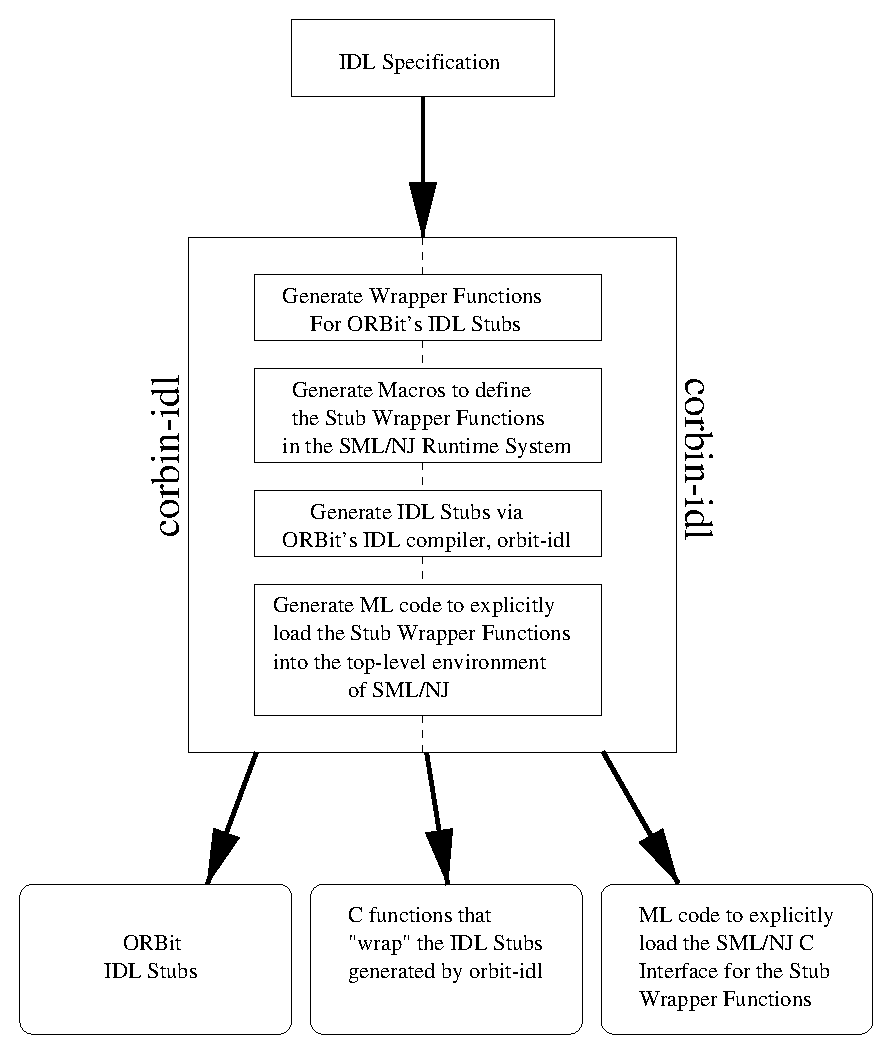
\psfig{file=Figures/corbinIDLStubs.eps}
\leavevmode
\caption{\em{Diagram of the corbin-idl stub generation process}.}
\figline
         \label{corbinIDLStubs}
\end{center}
\end{figure}

\subsection*{IDL skeletons}
\addcontentsline{toc}{subsection}{IDL skeletons} 

The first step in the corbin-idl skeleton generation process involves the 
generation of C function pointers.  These function pointers are used to 
retain references to ML functions.  When a request is received by 
ORBit to invoke an operation, the function pointers can be used 
to call the ML function that implements the requested operation. 
The function pointer generated for the foo object's bar operation is 
listed in figure \ref{CFunToML}.
\begin{figure*}[t]
\singlespace
\begin{verbatim}

  long (*CORBin_foo_bar_MLFn)(long );

\end{verbatim}
\doublespace
\caption {\em{C function pointer used to call the ML function that implements the foo object's bar operation}.}
\figline
        \label{CFunToML}
\end{figure*}

Once function pointers have been generated for all operations in the IDL
specification, corbin-idl generates C functions that are included in the 
SML/NJ runtime system so that the ML programmer can assign to these function 
pointers the address of the ML function that implements the corresponding 
operation. The C function generated by corbin-idl to save a pointer to 
the ML function that implements the foo object's bar operation is listed 
in figure \ref{CSaveMLPtr}.
\begin{figure*}[t]
\singlespace
\begin{verbatim}

  void CORBin_foo_bar_SetMLFn(long  (*f)(long ))
  {
       CORBin_foo_bar_MLFn = f;
  }

\end{verbatim}
\doublespace
\caption {\em{C function used to save a pointer to the ML function that implements the foo object's bar operation}.}
\figline
        \label{CSaveMLPtr}
\end{figure*}

Having generated the function pointer assignment functions, 
corbin-idl now generates C functions to {\em{callback}} the appropriate 
ML function.   
These functions are called when ORBit receives a request to invoke
an operation on an object.  So, when a request is received and this function 
is called, it simply passes the parameters of interest along to the function
implemented by the ML programmer.  The C function generated by corbin-idl 
to {\em{callback}} the ML function that implements the foo object's bar 
operation is shown in figure \ref{CCallBackToML}.
\begin{figure*}[t]
\singlespace
\begin{verbatim}

  static long
  impl_foo_bar(impl_POA_foo * servant , long x, 
               CORBA_Environment * ev)
  {
     return CORBin_foo_bar_MLFn(x);
  }

\end{verbatim}
\doublespace
\caption {\em{C function generated by corbin-idl that is called by ORBit when a client application invokes the bar operation on the foo object}.}
\figline
        \label{CCallBackToML}
\end{figure*}

Once corbin-idl has generated the necessary C functions for the IDL skeletons, 
it must generate C macros to explicitly define the functions that must be 
accessible from the SML/NJ runtime system.  Since the function pointer
assignment functions are the only functions that the ML programmer must be 
able to call explicitly, we only need to generate macros to define those 
functions.  The C macro generated by corbin-idl for the 
CORBin\_foo\_bar\_SetMLFn function is listed in figure \ref{CMLFnMacro}. 
\begin{figure*}[t]
\singlespace
\begin{verbatim}

     C_CALLS_CFUNC("CORBin_foo_bar_SetMLFn",
                    CORBin_foo_bar_SetMLFn, 
                    void , (long  (*f)(long )  ))

\end{verbatim}
\doublespace
\caption {\em{C Macro to explicitly define the CORBin\_foo\_bar\_SetMLFn function in the SML/NJ runtime system}.}
\figline
        \label{CMLFnMacro}
\end{figure*}
In order to produce C code to marshall and de-marshall parameters for the 
skeleton related functions generated by corbin-idl, orbit-idl is now executed. 

Just like the corbin-idl stub generation process, we must now generate 
ML code to explicitly load all of the necessary functions that have been 
generated into the top-level environment of SML/NJ.  Also, since 
the function pointer assignment functions are the only functions generated 
during this process that the ML programmer must have the ability to call, 
we are only concerned with them during this step.  First, we must generate
ML signatures for each of the applicable functions.  The ML signature 
generated for CORBin\_foo\_bar\_SetMLFn is listed in figure \ref{CFunToMLSig}.
\begin{figure*}[t]
\singlespace
\begin{verbatim}

     val CORBin_foo_bar_SetMLFn : (cdata list -> cdata) ->  unit

\end{verbatim}
\doublespace
\caption {\em{ML signature for the CORBin\_foo\_bar\_SetMLFn function}.}
\figline
        \label{CFunToMLSig}
\end{figure*}
Following the generation of signatures, corbin-idl generates value/function 
pairs for the appropriate functions.  
\pagebreak
Figure \ref{MLSetFnValFun} lists 
the ML code generated during this step for the CORBin\_foo\_bar\_SetMLFn
function.   
\begin{figure*}[t]
\singlespace
\begin{verbatim}

val CORBin_foo_bar_SetMLFn' =
     registerAutoFreeCFn("CORBin_foo_bar_SetMLFn", 
                         [CfunctionT([ClongT], ClongT)],CvoidT)
fun CORBin_foo_bar_SetMLFn f =
     let val  Cvoid  = 
              CORBin_foo_bar_SetMLFn' [Cfunction f] 
     in  
         ()
     end

\end{verbatim}
\doublespace
\caption {\em{ML value/function pair for the CORBin\_foo\_bar\_SetMLFn function}.}
\figline
        \label{MLSetFnValFun}
\end{figure*}
These key steps in the corbin-idl skeleton generation process are illustrated 
in figure \ref{corbinIDLSkels}. 
\begin{figure}
\begin{center}
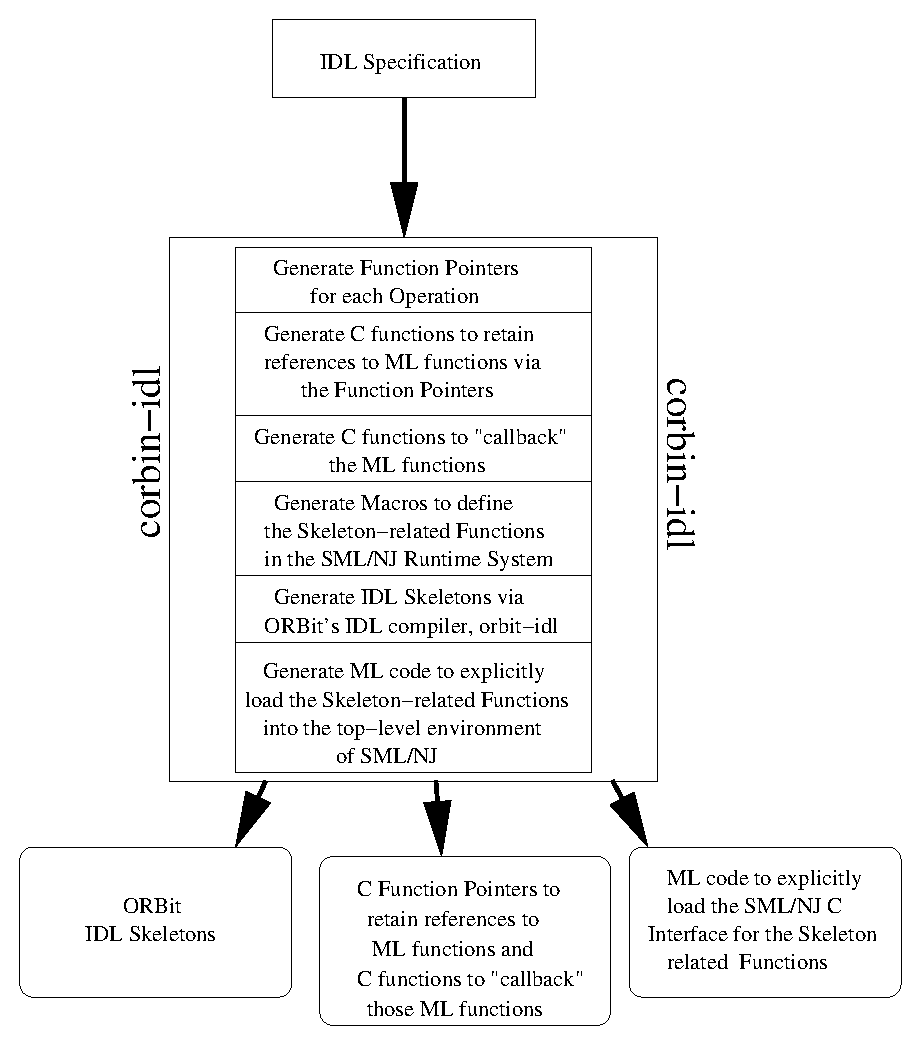
\psfig{file=Figures/corbinIDLSkels.eps}
\leavevmode
\caption{\em{Diagram of the corbin-idl skeleton generation process}.}
\figline
         \label{corbinIDLSkels}
\end{center}
\end{figure}

\newpage
\section*{\underline{The Library}}
\addcontentsline{toc}{section}{The Library}

The CORBin Library makes up the other half of the C ORB Interface System.
This library of C functions is combined with the SML/NJ runtime system in 
order to give ML programmers the ability to utilize ORBit's CORBA 
functionality.  This concept is illustrated in figure \ref{CORBinVisual}. 
\begin{figure}
\begin{center}
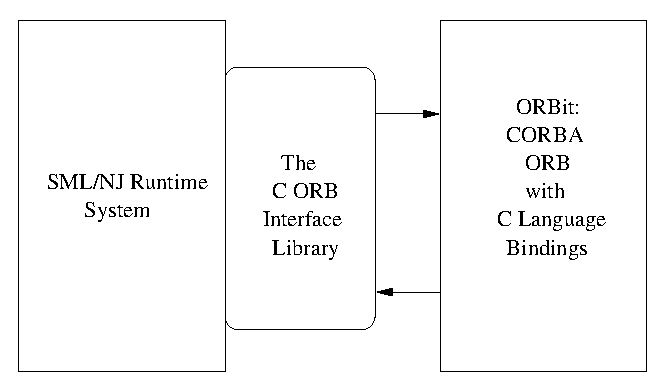
\psfig{file=Figures/CORBinVisual.eps}
\leavevmode
\caption{\em{The C ORB Interface Library}.}
\figline
         \label{CORBinVisual}
\end{center}
\end{figure}
The C functions in this library provide a standard interface 
to routines that already exist in ORBit.  They allow the ML programmer 
to use the most basic of ORBit's functionality and also the CORBA Name 
Service.  The basic routines that make up the CORBin Library are listed 
in figure \ref{CorbinLibrary}.  In addition to these basic routines, 
corbin-idl adds the necessary IDL stub and skeleton routines to this 
library when it processes IDL specifications.   
\begin{figure}
\begin{center}
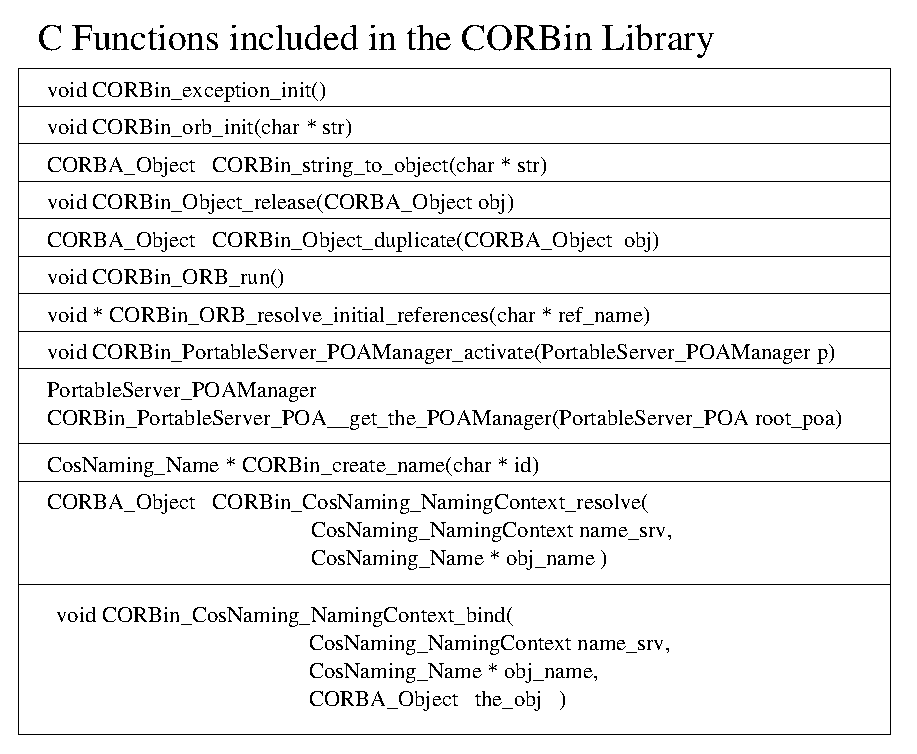
\psfig{file=Figures/CorbinLibrary.eps}
\leavevmode
\caption{\em{C Functions that make up the CORBin Library}.}
\figline
         \label{CorbinLibrary}
\end{center}
\end{figure}




%%%%%%%%%%%%%%%%%%%%%%%%%%%%%%%%%SYRUP Discussion%%%%%%%%%%%%%%%%%%%%%%%
\chapter{\uppercase{Case Study: An Instant Messaging Application}}
\label{study}

In recent years, the popularity of the Internet has soared. 
One of the more popular uses of the Internet is instant messaging. 
In this chapter, a distributed instant messaging system 
is presented to illustrate the use of the C ORB Interface 
System with the Standard ML of New Jersey compiler. 

\section*{\underline{SYRUP: Simple Yet Reliable Utility for Product Planning}}
\addcontentsline{toc}{section}{SYRUP: Simple Yet Reliable Utility for Product Planning}

Suppose a group of young entrepreneurs would like to start a 
corporation.  Also suppose that these young entrepreneurs live very 
far apart.  Since they live so far apart, meeting in person is simply 
not practical.  They also don't have a lot of money to waste on long 
distance telephone calls.  Therefore, they need some other means by which 
to communicate.  Since, Internet instant messaging provides a cost-effective 
solution to their dilemma, they elect to create their own instant messaging 
system that they can use to plan their corporate strategy and product line.   
In addition to the need for instant messaging capability, they would also 
like this application to provide the ability to post ideas on a message 
board that is accessible via a web browser.   

This scenario involving the young entrepreneurs provides an excellent 
opportunity to create a CORBA based application.  Since each entrepreneur 
could be using a different computing platform, we need to make sure 
that we can create components that can inter-operate with ease.  CORBA 
provides us with that ability.  Since there are many programming languages 
that can take advantage of CORBA capabilities, we need to select the 
language or languages that provide the most capability in the domain of 
our problem.  Because the distribution of the instant messaging application
will also be a concern, it would be nice if we could take advantage of 
JAVA's Applet facilities.  This way, the only software needed on each 
entrepreneur's computer is a web browser.  JAVA will also provide 
our client application with elegant graphical user interface features. 
Now that we have decided to implement our client application in JAVA, 
we must decide which programming language to use in the implementation 
of our instant messaging server.  This component will be responsible 
for maintaining a list of users that are currently using the system 
and are accepting instant messages.  It will also be responsible for 
passing instant messages from one user to another and writing messages 
on the message board.    Since ML offers a built-in list data type and 
a rich set of list manipulation features, the instant messaging server 
is an excellent opportunity to use the CORBin System to implement a 
CORBA object in ML.  
A diagram of the S$.$Y$.$R$.$U$.$P$.$ System is illustrated in figure 
\ref{SyrupComponentDiagram}.  
\begin{figure}
\begin{center}
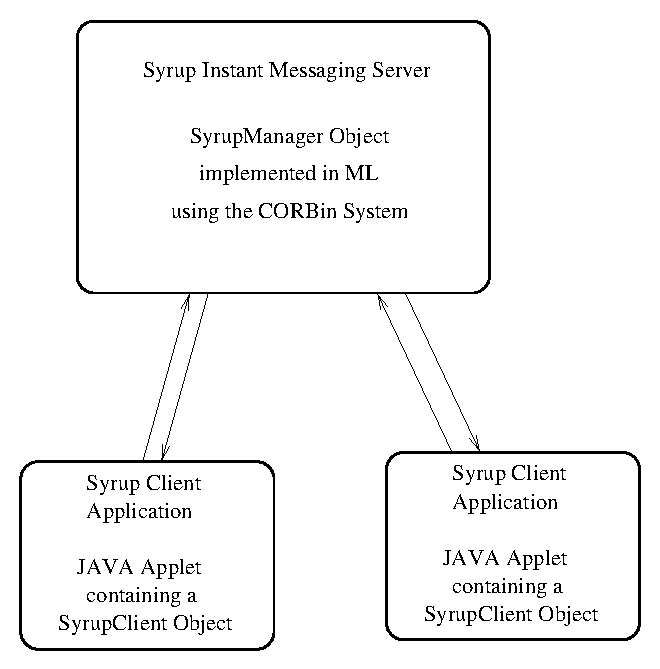
\psfig{file=Figures/SyrupComponentDiagram.eps}
\leavevmode
\caption{\em{Diagram of the S$.$Y$.$R$.$U$.$P$.$ System}.}
\figline
         \label{SyrupComponentDiagram}
\end{center}
\end{figure}

Notice that the instant messaging server must have the ability to 
communicate with each client application in addition to serving 
client application requests.   This also provides an excellent 
opportunity use a CORBA design pattern called {\em{callback}}. 
Using the CORBA callback pattern, the client application will pass 
a reference to a CORBA object to another CORBA object.  The receiving 
object can then retain the object reference to later invoke 
operations on it. Therefore, in addition to communicating with a remote CORBA
object, our client application will also contain a CORBA object that the 
instant messaging server can invoke operations on.  
Since we are using the callback pattern, the CORBA object we implement in ML
will not only illustrate how to use the CORBin system can be used to 
implement CORBA objects, it will also allow us to illustrate how ML 
can communicate with remote CORBA objects.

\section*{\underline{The Design}}
\addcontentsline{toc}{section}{The Design}

Before we can create an IDL specification for our application, we must 
determine what functionality is needed by our CORBA objects.  Clearly, 
we need some means by which users can register and unregister themselves
as S$.$Y$.$R$.$U$.$P$.$ users.  Therefore, our SyrupManager object should 
have the ability to allow users to {\em{Login}} and {\em{Logout}}.  
Also, it should provide functionality to allow users to {\em{send messages}} 
to one another. As a final requirement, the SyrupManager object should allow 
users to {\em{post messages}} to an electronic bulletin board.  These 
ideas are illustrated using the Unified Modeling Language (UML) in figure 
\ref{SyrupManagerUseCases}. 
\begin{figure}
\begin{center}
\psfig{file=Figures/SyrupManagerUseCases.eps}
\leavevmode
\caption{\em{UML Use Cases for the SyrupManager Object}.}
\figline
         \label{SyrupManagerUseCases}
\end{center}
\end{figure}

The SyrupManager object also requires some functionality to be included 
in the SyrupClient object.  First, The SyrupManager needs 
to be able to add and remove users from a list of users that are currently 
available to receive instant messages.  In addition to these requirements, 
the SyrupClient object must also include functionality to allow for the 
delivery of instant messages. These ideas are also illustrated using UML in 
figure \ref{SyrupClientUseCases}.
\begin{figure}
\begin{center}
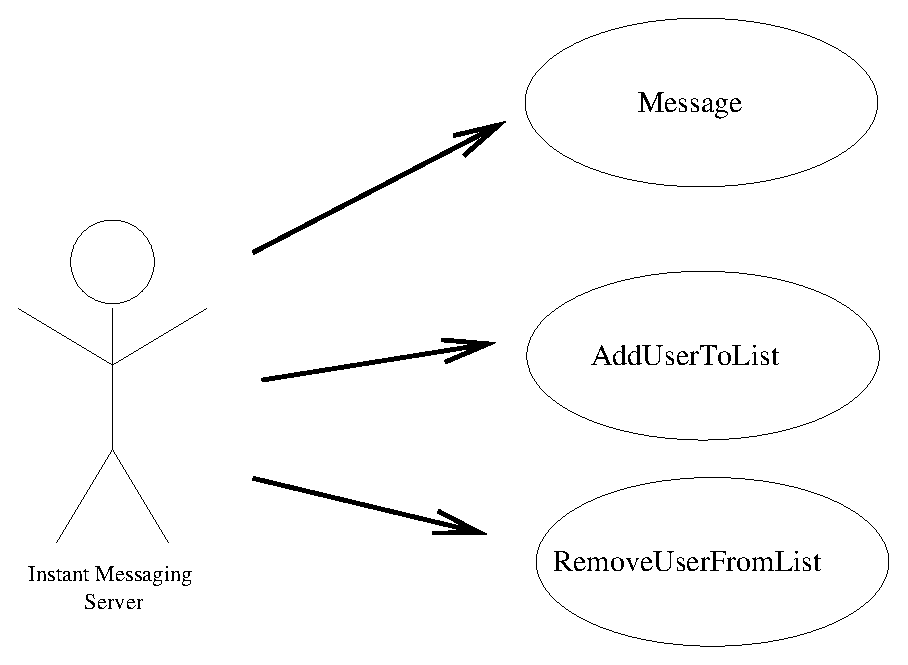
\psfig{file=Figures/SyrupClientUseCases.eps}
\leavevmode
\caption{\em{UML Use Cases for the SyrupClient Object}.}
\figline
         \label{SyrupClientUseCases}
\end{center}
\end{figure}

Now that we know the required functionality of each object, we can construct 
UML class diagrams that illustrate the necessary parameters and their types for 
each operation.  The operations that belong to the SyrupManager object are 
shown in figure \ref{SyrupManagerClassDiagram} and the operations that belong 
to the SyrupClient object are shown in figure \ref{SyrupClientClassDiagram}.   
Notice that the {\em{Login}} operation of the SyrupManager object requires two 
parameters: a string representing a user name and a reference to a SyrupClient 
object.  This allows the SyrupManager object to send updates back to that 
client application.
\begin{figure}
\begin{center}
\psfig{file=Figures/SyrupManagerClassDiagram.eps}
\leavevmode
\caption{\em{UML Class Diagram for the SyrupManager Object}.}
\figline
         \label{SyrupManagerClassDiagram}
\end{center}
\end{figure}
\begin{figure}
\begin{center}
\psfig{file=Figures/SyrupClientClassDiagram.eps}
\leavevmode
\caption{\em{UML Class Diagram for the SyrupClient Object}.}
\figline
         \label{SyrupClientClassDiagram}
\end{center}
\end{figure}


\section*{\underline{Interface Definition}} 
\addcontentsline{toc}{section}{Interface Definition}

Recall that before we can implement a CORBA object in a programming 
language, we must define the interface by which other CORBA objects 
may utilize our object's functionality. The IDL specification for 
our instant messaging application is listed in figure \ref{syrupIDL}.
Notice the use of the IDL keyword {\em{oneway}}.
Here, we use the {\em{oneway}} keyword when we do not want to wait on 
the operation to return before we can continue processing.  This 
{\em{oneway}} feature of CORBA is implemented in various degrees 
of robustness by ORB vendors. It should be noted that if you must 
know that the parameters were correctly received by the remote 
object then the {\em{oneway}} attribute should probably not be used. 
Upon completion of the IDL specification, corbin-idl is used to 
generate IDL stubs, IDL skeletons, and rebuild the SML/NJ runtime 
system. 
\begin{figure*}[t]
\singlespace
\begin{verbatim}

  module Syrup {

        interface SyrupClient  {

                oneway void Message(in string userid, 
                                    in string msg);	
                oneway void AddUserToList(in string userid); 
                oneway void RemoveUserFromList(in string userid); 
        };

        interface SyrupManager {
	
                void Login  (in string userid, 
                             in SyrupClient client); 
                void Logout (in string userid);		
                oneway void PostMessage (in string userid, 
                                         in string msg);
                oneway void SendMessage (in string from, 
                                         in string to,
                                         in string msg);

        };

  };

\end{verbatim}
\doublespace
\caption {{\em IDL specification for the S$.$Y$.$R$.$U$.$P$.$ Instant Messaging Application}.}
\figline
        \label{syrupIDL}
\end{figure*}



\section*{\underline{IDL Skeleton Implementation}}
\addcontentsline{toc}{section}{IDL Skeleton Implementation}

Once we have compiled the IDL specification for our application, we must 
implement the CORBA objects in a programming language.  In this case, we
must implement the operations of the SyrupManager object in ML so that 
a client application can use it to communicate with other Syrup users. 
The ML code used to implement the SyrupManager operations is listed in 
figure \ref{SyrupManagerInML}. 
\begin{figure*}[t]
\singlespace
\begin{verbatim}


fun Login [Cstring id, Caddr obj] = 
          (SyrupManager.add_user_to_list(id,obj);
           Cint(0w1) )
fun Logout [Cstring id] = 
          (SyrupManager.remove_user_from_list(id);
           Cint(0w1) )
fun PostMessage [Cstring id, Cstring msg] = 
          (SyrupManager.write_message(id, msg);
           Cint(0w1) )

fun SendMessage [Cstring from, Cstring to, Cstring msg] = 
          (SyrupManager.send_message(from,to, msg);
           Cint(0w1) )

val _ = CORBin_Syrup_SyrupManager_Login_SetMLFn(Login);
val _ = CORBin_Syrup_SyrupManager_Logout_SetMLFn(Logout);
val _ = CORBin_Syrup_SyrupManager_PostMessage_SetMLFn(PostMessage);
val _ = CORBin_Syrup_SyrupManager_SendMessage_SetMLFn(SendMessage);

\end{verbatim}
\doublespace
\caption {{\em SyrupManager Implementation in ML}.}
\figline
        \label{SyrupManagerInML}
\end{figure*}
Notice that each function takes a list as a parameter.  This list is 
composed of data types defined in a SML/NJ library that accompanies the 
SML/NJ C interface.  These data types represent their counterparts in the 
C programming language.  Also notice that although these functions were defined 
to have no return value in the IDL specification, the CORBin System requires 
that void functions return an integer value.  In order to modularize 
our implementation of the SyrupManager object, a separate ML structure has 
been defined that contains various utility functions.  Excerpts from this 
structure are listed in figure \ref{SyrupManagerStructure}.  The full 
source code listing for the SyrupManager structure is presented in the 
appendix.   
\begin{figure*}[t]
\singlespace
\begin{verbatim}

val user_list: (string * caddr) list ref  = ref []

fun add_user_to_clients_gui(id: string, nil) =  ()
  | add_user_to_clients_gui(id: string, 
                          (uid: string, obj: caddr)::rest) =
    (if (id = uid) then
        add_user_to_clients_gui(id, rest)
     else
        (CORBin_Syrup_SyrupClient_AddUserToList(obj, id);
         add_user_to_clients_gui(id, rest)))

fun add_users_to_new_clients_gui(obj: caddr, nil) =  ()
  | add_users_to_new_clients_gui(obj: caddr,
                          (uid: string, uobj: caddr)::rest) =
    (CORBin_Syrup_SyrupClient_AddUserToList(obj, uid);
     add_users_to_new_clients_gui(obj, rest))


fun add_user_to_list (id: string, obj: caddr) =
    let val obj_copy = CORBin_Object_duplicate(obj)
    in
          user_list := (id,obj_copy)::(!user_list);
          add_user_to_clients_gui(id, !user_list);
          add_users_to_new_clients_gui(obj_copy, !user_list)
    end

\end{verbatim}
\doublespace
\caption {{\em Excerpts from an ML structure providing utility functions to our SyrupManager implementation}.}
\figline
        \label{SyrupManagerStructure}
\end{figure*}

In order to illustrate the process of implementing a CORBA object in ML using 
the CORBin System, we will now discuss the Login operation of the SyrupManager 
object in detail.  In figure \ref{SyrupManagerInML}, you will notice that the 
the Login operation calls a function, {\em{add\_user\_to\_list}}, that is 
defined in a structure called SyrupManager.
The code for this function is listed in figure \ref{SyrupManagerStructure}.   
Notice that {\em{add\_user\_to\_list}} first calls {\em{CORBin\_Object\_duplicate}} 
to increment the reference count for the object reference of the SyrupClient 
object we received from the client application.  This is done since ORBit 
object references maintain a reference count in order to determine if they are 
still in use.   Once this has been done, we add the string representing the 
user's screen name and the SyrupClient object reference to a list as a tuple.  
Now, we must notify other users that a new user has just logged in to the system. 
The reason this is of interest is because it illustrates how ML programmers can 
communicate with other CORBA objects with the CORBin System.  Notice that the 
first line of the {\em{add\_user\_to\_clients\_gui}} function is a call to the 
{\em{CORBin\_Syrup\_SyrupClient\_AddUser\-ToList}} function.  This should look somewhat
familiar as this function was generated by corbin-idl when the IDL specification
for the S$.$Y$.$R$.$U$.$P$.$ application was processed.  As with all CORBin related 
functions, this function name begins with CORBin.  The rest of the name is composed 
of {\em{module name}} (Syrup), {\em{interface name}} (SyrupClient), and 
then {\em{operation name}} (AddUserToList).  Each name is separated by the underscore
character.  The object reference for the remote object is always the first parameter
passed to an IDL stub function generated by corbin-idl. Any additional parameters 
are passed after the object reference in the order in which they are defined in the 
IDL specification.   This naming convention is used for all IDL stub functions 
generated by corbin-idl.  Now that the Login operation has been implemented in ML, 
we must register it with the CORBin System so that client applications may utilize it.
This is done by passing the name of the function that implements the operation to 
a function generated by corbin-idl.  This function saves a pointer to the ML function 
that implements the operation so that when requests arrive to execute the operation, 
this function pointer is used to execute the ML code necessary to complete the operation.   
In order to establish that the ML function {\em{Login}} implements the Login operation
of the SyrupManager object, we call the {\em{CORBin\_Syrup\_SyrupManager\_Login\_SetMLFn}}
function. The naming convention for these function registration routines is similar 
to the IDL stub functions except {\em{SetMLFn}} is appended to the end of the function 
name.  Before activating a CORBA object implemented using the CORBin System, 
the programmer should always register a function that implements each operation 
defined for the object. 

Once the ML programmer has implemented the operations of a CORBA object with 
ML functions and registered those functions, some additional work must be done 
before this object can be used by a client application.  The code needed to 
{\em{activate}} our SyrupManager implementation in ML is listed in figure 
\ref{MLObjectActivate}. This setup process should look familiar to experienced 
CORBA developers.  This process involves creating a SyrupManager object, activating 
the Portable Object Adapter (POA), and publishing our SyrupManager's object 
reference to a name service.  If the reader is new to CORBA and CORBA development, 
the author suggests that a CORBA text book be referenced to better understand 
this process and why it must be done before the object implementation may 
be utilized.  
\begin{figure*}[t]
\singlespace
\begin{verbatim}

val naming_ior = "-ORBNamingIOR=IOR:<<IOR of Name Service...>>";

val x = CORBin_exception_init() ;

val x = CORBin_orb_init (naming_ior);

val root_poa = CORBin_ORB_resolve_initial_references("RootPOA");
val poa_man = 
        CORBin_PortableServer_POA__get_the_POAManager(root_poa);

val _ = CORBin_PortableServer_POAManager_activate(poa_man);

val manager = CORBin_Syrup_SyrupManager_create(root_poa);

val name_srv = 
    CORBin_ORB_resolve_initial_references("NameService");

val manager_name = CORBin_create_name("SyrupManager");

val _ = CORBin_CosNaming_NamingContext_bind(name_srv, 
                                            manager_name, 
                                            manager);

val _ = CORBin_ORB_run();
 
\end{verbatim}
\doublespace
\caption {{\em Code to activate the SyrupManager object implementation in ML}.}
\figline
        \label{MLObjectActivate}
\end{figure*}

Once the SyrupManager object has been activated, it can be utilized
by a client application.  In this case study, a client application was written 
in JAVA.  A screen capture of this application in use is shown in figure 
\ref{SyrupScreenShot}.  The source code for this JAVA application can be found in 
the appendix.
\begin{figure}
\begin{center}
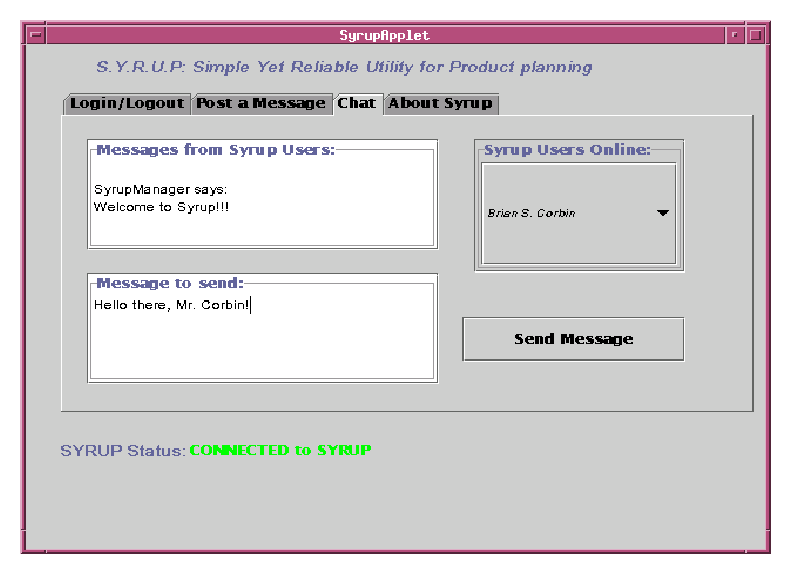
\psfig{file=Figures/syrup_screen_shot.eps}
\leavevmode
\caption{\em{Screen Capture of a SYRUP client application implemented in JAVA}.}
\figline
         \label{SyrupScreenShot}
\end{center}
\end{figure}

\section*{\underline{Performance}}
\addcontentsline{toc}{section}{Performance}

One factor that can influence the selection of an implementation language for a 
CORBA object is performance.  Clearly, we would like for our CORBA objects to
respond as quickly as possible to client application requests.  While this response
time is greatly influenced by the ORB in use, the implementation language can 
play a factor in how quickly operations are executed.  In this section, 
we conduct a performance experiment to compare two different implementations 
of the SyrupManager object using the same Object Request Broker, ORBit.   

\subsection*{The Experiment}
\addcontentsline{toc}{subsection}{The Experiment}

In order to determine if CORBA objects implemented in ML can provide 
satisfactory performance,  the SyrupManager object was re-implemented in C.
A Java application was written to repeatedly invoke the Login and Logout 
operations of the SyrupManager object and report the average time it took 
to execute the each operation.  The Java application was executed on a 
Sparc Ultra 5 with 128 Megabytes of physical memory running Solaris 7 using the 
Java Runtime Environment 1.3.  Both implementations of the SyrupManager 
object were executed on a PC with a Pentium 166 MHz processor and 64 Megabytes 
of physical memory running RedHat Linux 6.2.  ORBit version 0.5.6 was used 
as the Object Request Broker for both implementations. The C version of the 
SyrupManager object was compiled with gcc version 2.91.66. (No optimizations 
were used.)  


\subsection*{Experiment Results}
\addcontentsline{toc}{subsection}{Experiment Results}

The results from the experiment are shown in figure \ref{PerformanceResults}.
As the figure indicates, the ML implementation offers performance parallel to the 
C implementation.  As the number of invocations increases, it seems as though the 
C implementation performs slightly better on average.  This performance difference 
could be attributed to ML garbage collection.  
\begin{figure}
\begin{center}
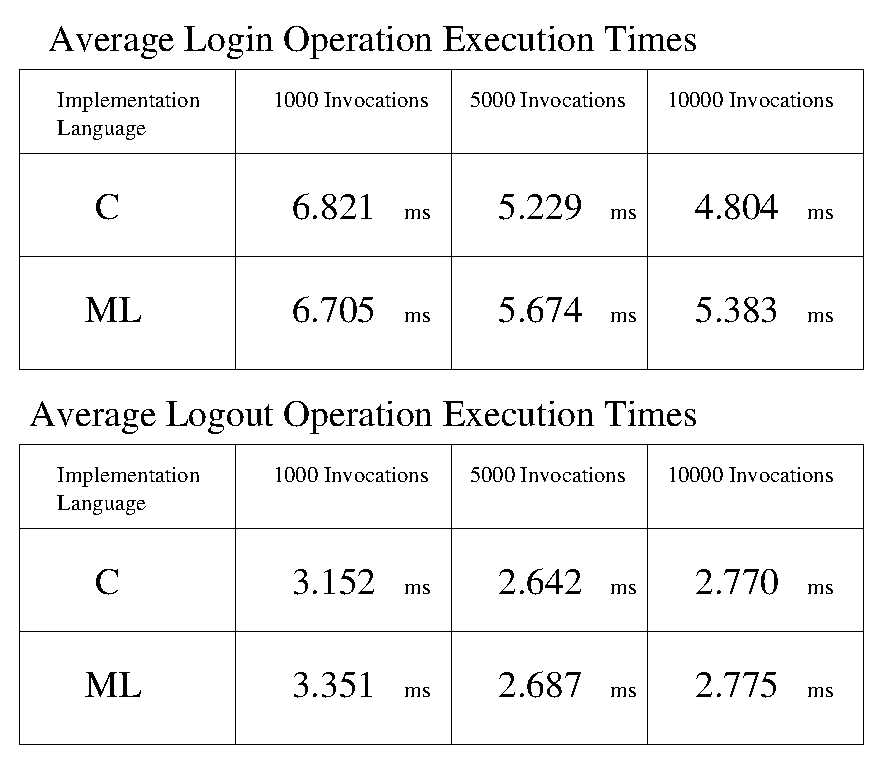
\psfig{file=Figures/PerformanceResults.eps}
\leavevmode
\caption{\em{Timings for Login and Logout operation invocations on two different implementations of the SyrupManager object}.}
\figline
         \label{PerformanceResults}
\end{center}
\end{figure}




%%%%%%%%%%%%%%%%%%%%%%%%%%%%%%%%Summary%%%%%%%%%%%%%%%%%%%%%%%%%%%%%%
\chapter{\uppercase{Summary}}
\label{summary}

We have designed and implemented an interface system (CORBin) 
to work with ORBit, a freely available ORB with C language 
bindings, in order to provide CORBA support for the functional 
language, ML. The interface system provides an IDL compiler, 
corbin-idl, that processes an Interface Definition Language 
(IDL) file and generates C functions which utilize the 
functionality provided by ORBit.  These C functions are 
added to a library that is compiled into the SML/NJ runtime 
system.  The resulting runtime system provides the ML programmer 
with the ability to implement and communicate with CORBA objects 
defined within the IDL file.  A case study was presented to 
illustrate the use of the CORBin System in the development of 
a distributed instant messaging application.   A performance
experiment was conducted to show that CORBA objects implemented
in ML using the CORBin System can achieve satisfactory performance
levels for operation execution.   The performance experiment compared
two different implementations of a CORBA object.  One version was 
implemented in C and another was implemented in ML using the CORBin
System.  The average execution times for the operations 
invoked by a client application were roughly the same for both 
implementations.  The source code for the CORBin System,
case study,  and performance test can be retrieved from
{\em{http://www.corbinator.com}}.  



While the C ORB Interface has been used to implement and communicate 
with CORBA objects, it should still be considered a prototype.   
Currently, the C functions generated by corbin-idl are compiled 
into a static library and linked into the SML/NJ runtime system.  
Future work could involve modifying corbin-idl to work with a 
dynamic, shared library in order to avoid re-compilation of the 
entire SML/NJ runtime system.

Since corbin-idl has been implemented in ML and uses modular 
programming techniques, it could easily be extended to provide 
CORBA support for other programming languages that can call C 
functions.  This could provide a quick solution for providing 
CORBA support to programming languages without the need to 
implement a new ORB or provide additional language bindings 
for an existing ORB. 



%%%%%%%%%%%%%%%%%%%%%%%%%%%%%%%%Appendix%%%%%%%%%%%%%%%%%%%%%%%%%%%%%%%
\chapter{\uppercase{Appendix}}
\label{appendix}
\singlespace
\section*{\underline{The IDL Grammar}}
\addcontentsline{toc}{section}{The IDL Grammar}
\input{idl_gram}
\section*{\underline{S$.$Y$.$R$.$U$.$P$.$ Source Code Listing}}
\addcontentsline{toc}{section}{S$.$Y$.$R$.$U$.$P$.$ Source Code Listing}
\subsection*{ML implementation of the SyrupManager object}
\addcontentsline{toc}{subsection}{ML implementation of the SyrupManager object}
\begin{verbatim}

(* Must open these structures in order to use the ML/C Interface *)
open CI;
open CU;
(*****************************************************************)

use "SyrupManager.sml";

val naming_ior = "-ORBNamingIOR=<<<IOR of NameServer goes here!>>>";

(*****set function ptrs ****)

fun Login [Cstring id, Caddr obj] = 
    (SyrupManager.add_user_to_list(id,obj);
     Cint(0w1))

fun Logout [Cstring id] = 
    (SyrupManager.remove_user_from_list(id);
     Cint(0w1) )

fun PostMessage [Cstring id, Cstring msg] = 
    (SyrupManager.write_message(id, msg);
     Cint(0w1))

fun SendMessage [Cstring from, Cstring to, Cstring msg] = 
    (SyrupManager.send_message(from,to, msg);
     Cint(0w1))

val _ = CORBin_Syrup_SyrupManager_Login_SetMLFn(Login);
val _ = CORBin_Syrup_SyrupManager_Logout_SetMLFn(Logout);
val _ = CORBin_Syrup_SyrupManager_PostMessage_SetMLFn(PostMessage);
val _ = CORBin_Syrup_SyrupManager_SendMessage_SetMLFn(SendMessage);

val x = CORBin_exception_init() ;

val x = CORBin_orb_init (naming_ior);

val root_poa = 
    CORBin_ORB_resolve_initial_references("RootPOA");
val poa_man = 
    CORBin_PortableServer_POA__get_the_POAManager(root_poa);
val _ = CORBin_PortableServer_POAManager_activate(poa_man);

val manager = CORBin_Syrup_SyrupManager_create(root_poa);

val name_srv = CORBin_ORB_resolve_initial_references("NameService");

val manager_name = CORBin_create_name("SyrupManager");

val _ = CORBin_CosNaming_NamingContext_bind(name_srv, 
                              manager_name, manager);

print "Ready to serve requests!\n\n";
val _ = CORBin_ORB_run(); 


\end{verbatim}
     
\subsection*{ML SyrupManager Structure with Utility Functions}
\addcontentsline{toc}{subsection}{ML SyrupManager Structure with Utility Functions}
\input{ml_impl_utility}     


%\subsection{C implementation of the SyrupManager object}
%\input{c_impl}
%\subsection{S$.$Y$.$R$.$U$.$P$.$ Client Application implemented in JAVA}
%\input{java_client}
%\section{Performance Experiment Code Listing}
%\subsection{Java application source code}



\doublespace


%
% The following two commands are all you need in the
% initial runs of your .tex file to
% produce the bibliography for the citations in your paper.

\newpage
\bibliographystyle{plain}
\bibliography{paper}  % paper.bib is the name of the Bibliography

% And that's the bottom line ... cause it's "Miller Time!"
\end{document}
